% Manual of pgf-pie.sty, a convenient set of macros for drawing pie
% chart. Written by Xu Yuan <xuyuan.cn@gmail.com> This file is part of
% pgf-pie you may get it at https://github.com/pgf-tikz/pgf-pie

\PassOptionsToPackage{%
  colorlinks=true,
  linkcolor=blue,
  anchorcolor=black,
  citecolor=olive,
  filecolor=magenta,
  menucolor=red,
  urlcolor=blue
}{hyperref}
\documentclass{ltxdoc}

\usepackage{pgf-pie}
\usetikzlibrary{babel, shadows}

\usepackage[a4paper,left=2.25cm,right=2.25cm,top=2.5cm,bottom=2.5cm,nohead]{geometry}
\usepackage{calc}
\usepackage{graphicx}
\input{pgfmanual-en-macros.tex}

\pgfqkeys{/codeexample}{%
  scale/.store in=\pgfpieexamplescale,
  scale=1,
  every codeexample/.style={%
    width=.4\textwidth+7pt,
    pre={
      \setbox\codeexamplebox=\hbox\bgroup
    },
    post={
      \egroup
      \resizebox{\pgfpieexamplescale\textwidth}{!}{\box\codeexamplebox}%
    },
  },
}

\newcommand\pgfpiename{\texttt{pgf-pie}}

\begin{document}

\title{Drawing Pie Chart by using \pgfpiename}
\author{\href{mailto:xuyuan.cn@gmail.com}{Yuan Xu}}
\date{\today{}~(v0.7)}
\maketitle

\begin{abstract}
  \pgfpiename\ is a LaTeX package for drawing pie chart (and
  variant charts). As stated by its name, it is based on a very
  popular graphic package \pgfname/\tikzname. This document presents
  the usage of \pgfpiename\ and collects some pie charts as
  examples. \pgfpiename\ can be downloaded from
  \href{https://github.com/pgf-tikz/pgf-pie}{https://github.com/pgf-tikz/pgf-pie}.
\end{abstract}

\tableofcontents

\section{Usage}

\subsection{First Pie}
|\pie| is the only command that provided by
\pgfpiename. The argument is a list of number and text
combination in the formate of |number/text|, i.e. |10/A, 20/B, 30/C, 40/D|.
The result is shown in figure \ref{fig:first-pie}.
\begin{figure}
  \centering
  \codeexample[scale=0.25,from file={demo/first-pie.tex}]
  \caption{The first pie.}
  \label{fig:first-pie}
\end{figure}

\subsection{Position, Rotation, Size}

The center of chart can be set by |pos|, default is
|{0,0}|. The chart can be rotated by setting |rotate|
(in degrees). The size of chart can be set by |radius|, default
is 3.

\codeexample[scale=0.4,from file={demo/radius.tex}]

\subsection{Color}
The color can be specified by |color|, the default color wheel
is shown in figure \ref{fig:color-wheel}.
\begin{figure}
  \centering
  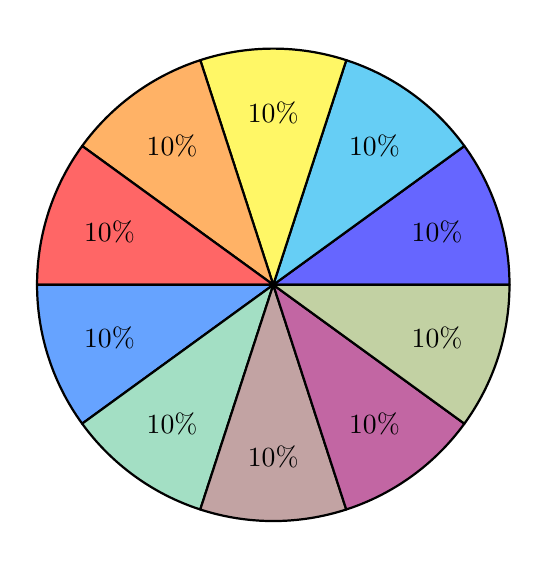
\begin{tikzpicture}
  \pie{10/, 10/, 10/, 10/, 10/, 10/, 10/, 10/, 10/, 10/}
\end{tikzpicture}
  \caption{Default color wheel}
  \label{fig:color-wheel}
\end{figure}

\codeexample[scale=0.4,from file={demo/color.tex}]

\subsection{Explode}
\codeexample[scale=0.4,from file={demo/explode.tex}]

\subsection{Angle of slices}
The value of |sum| indicates the sum of all data in the chart,
it is 100 by default. It can be calculated automatically when
|auto| is set. Then the angle of slices are determined by
number value and |sum|.

\codeexample[scale=0.4,from file={demo/sum.tex}]

\subsection{Slice order}
The slices order direction can be set to clockwise by setting |change direction|, default is counterclockwise.

\codeexample[scale=0.4,from file={demo/change-direction.tex}]

\subsection{Text}

\subsubsection{Number}
Two parameters can be used to decorate number: |before number|
and |after number|. Both are empty by default, but if
|sum=100|, |after number| will be set to \%
automatically if user doesn't set it.

\codeexample[scale=0.25,from file={demo/before-after-number.tex}]

The number also can be hide by |hide number|:

\codeexample[scale=0.25,from file={demo/hide-number.tex}]

\paragraph{Scale font}
The size of font in size pie can be scaled according to how big the
part is automatically.

\codeexample[scale=0.25,from file={demo/scalefont.tex}]

\subsubsection{Label text}
The value of |text| can be |label| (default),
|pin|, |inside| or |legend|.

\codeexample[scale=0.25,from file={demo/text.tex}]

\codeexample[scale=0.25,from file={demo/text-inside.tex}]

\codeexample[scale=0.25,from file={demo/legend.tex}]

\subsection{More about style}
\subsubsection{shadow}
\codeexample[scale=0.25,from file={demo/shadow.tex}]

\section{Variant Charts}
\subsection{Polar area diagram}
The polar area diagram is similar to a usual pie chart, except sectors
are equal angles and differ rather in how far each sector extends from
the center of the circle.

\codeexample[scale=0.25,from file={demo/polar.tex}]

\subsection{Square}

\codeexample[scale=0.25,from file={demo/square.tex}]

Note: |explode| has no affects in square chart.

\subsection{Clouds}

\codeexample[scale=0.25,from file={demo/cloud.tex}]

\section{Examples}

% \subsection{Population of the world}
% \example{population}

\section{Acknowledgements}
Many people contributed to \pgfpiename\ by reporting problems,
suggesting various improvements or submitting code. Here is a list of
these people:
\href{mailto:mohammed.alfaki@ii.uib.no}{Mohammed Alfaki},
and
\href{mailto:ldrude@mail.uni-paderborn.de}{Lukas Drude}
.
                                              
\end{document}
%%% Local Variables: 
%%% mode: Tex-PDF
%%% TeX-master: t
%%% End: 
